
Since we need to make our decisions about which variables to observe
before we know their values, we can only consider this quotient in
expectation.  and we can also consider the expected available energy
change,
\[
\expDist{\Delta E}{\trueProb(\dataVariables)} = T k_B\expDist{\log I}{\trueProb(\dataVariables)}.
\]
Now we are faced with the problem of approximating the available
energy because we don't have direct access to
$\trueProb(\dataVariables)$.

Our first approach will be to lower bound the expected intelligence
quotient. Introducing a variational distribution
$\simProb(\dataVariables)$, and considering the expected log
intelligence quotient under this distribution we have,
\[
\expDist{\log I}{\simProb(\dataVariables)}   = - \beta E(\measuredVariables_\dataVariables=\textbf{1}) - \expDist{\log \trueProb(\dataVariables)}{\simProb(\dataVariables)}
\]
which is lower bounded by,
\begin{equation}
  \expDist{\log I}{\simProb(\dataVariables)} \geq - \beta
  E(\measuredVariables_\dataVariables=\textbf{1}) - \expDist{\log
    \simProb(\dataVariables)}{\simProb(\dataVariables)}, \label{eqn-lir-lower}
\end{equation}
giving us a lower bound on the expected log intelligence quotient,
where the expectation is taken under the variational
distribution. Maximising this lower bound implies maximising the
entropy of $\simProb(\dataVariables)$. Unfortunately, the entropy is
unbounded. Which implies that the expected intelligence quotient under
a general distribution $\simProb(\dataVariables)$ is also
unbounded. We need more constraints on $\simProb(\cdot)$ to make
progress.

We can rewrite $\log \physicsProb(\dataVariables)$ as
\begin{align}
    \log \trueProb(\dataVariables) & =
    \expDist{\trueProb(\dataVariables,
      \stateVariables)}{\simProb(\stateVariables )} + \expDist{\log
      \simProb(\stateVariables)}{\simProb(\stateVariables)} +
    \text{KL}(\simProb(\stateVariables)||\trueProb(\stateVariables|\dataVariables))
    \nonumber \\ & = -\beta\expDist{ E(\dataVariables |
      \stateVariables)}{\simProb(\stateVariables)}
    -\beta\expDist{E(\stateVariables)}{\simProb(\stateVariables)} -
    \log Z_{\stateVariables,\dataVariables} + \expDist{\log
      \simProb(\stateVariables)}{\simProb(\stateVariables)} +
    \text{KL}(\simProb(\stateVariables)||\trueProb(\stateVariables|\dataVariables)) \label{eqn-true-log-likelihood-1}
\end{align}
and now note that
\[
- \log Z_{\stateVariables,\dataVariables} =
\beta\expDist{E(\dataVariables |
  \stateVariables)}{\simProb(\stateVariables)\trueProb(\dataVariables)}
+ \beta\expDist{E(\stateVariables)}{\simProb(\stateVariables )} -
k_B^{-1}S_\dataVariables -\expDist{\log
  \simProb(\stateVariables)}{\simProb(\stateVariables)} -
\expDist{\text{KL}(\simProb(\stateVariables) ||
  \trueProb(\stateVariables |
  \dataVariables))}{\trueProb(\dataVariables)}
\]
if we now define
\[
\physicsProb(\dataVariables) = \frac{\exp\left(-\beta
  \expDist{E(\dataVariables |
    \stateVariables)}{\simProb(\stateVariables)}\right)}{Z^\prime_\dataVariables}
\]
then we can write
\[
\log \trueProb(\dataVariables) = \log \physicsProb(\dataVariables) +
\text{KL}(\trueProb(\dataVariables)||\physicsProb(\dataVariables)) +
\text{KL}(\simProb(\stateVariables)||\trueProb(\stateVariables|\dataVariables))
-
\expDist{\text{KL}(\simProb(\stateVariables)||\trueProb(\stateVariables|\dataVariables))}{\trueProb(\dataVariables)}.
\]
so we can show that
\[
\log \trueProb(\dataVariables) \geq \log \physicsProb(\dataVariables)
-
\expDist{\text{KL}(\simProb(\stateVariables)||\trueProb(\stateVariables|\dataVariables))}{\trueProb(\dataVariables)}.
\]
Maximizing this lower bound is achieved through minimizing
$\expDist{\text{KL}(\simProb(\stateVariables)||\trueProb(\stateVariables|\dataVariables))}{\trueProb(\dataVariables)}$,
in other words, finding a variational distribution which represents
how the microstates behave correctly. Maximising this bound improves
the physical plausibility of the model. We call
$\simProb(\stateVariables)$ the \emph{simulation}\footnote{Because the paper bridges some different fields, and tries to equate
thermodynamic and information theoretic terms with words that are
widely used in modelling, it may be seen as abusing terminology in
parts. So to clarify at the outset, we are using some general terms in
very specific ways.

In particular, we use the word \emph{simulation} to imply a physical
model over the microstates of the universe that represents our 'best
practical' understanding of the underlying physics. In what follows
this simulation is denoted by
$\physicsProb(\stateVariables|\dataVariables)$. Alongside this we have
the \emph{data model}, which represents the marginal distribution for
the data we observe, $\physicsProb(\dataVariables)$. Quite often in
the below we will refer to this simply as `the model' as it will turn
out to be one of the main objects of focus.
} and we call
$\exp\left(-
\expDist{\text{KL}(\simProb(\stateVariables)||\trueProb(\stateVariables|\dataVariables))}{\trueProb(\dataVariables)}\right)$
the global simulation fidelity, $F_G$,
\[
\log F_G =
-\expDist{\text{KL}(\simProb(\stateVariables)||\trueProb(\stateVariables|\dataVariables))}{\trueProb(\dataVariables)}.
\]
Note that the fidelities we define vary between 0 and 1, with 1 being
equivalent to 100\% faithful, meaning that the match between the two
distributions is perfect.

This in turn gives us an upper bound on our log intelligence quotient,
\[
\log I \leq -\beta E(\measuredVariables_\dataVariables = \textbf{1})
-\log \physicsProb(\dataVariables) - \log F_G.
\]
So we can write the intelligence quotient as,
\[
I \leq
\frac{1}{F_G}\frac{\exp\left(-E(\measuredVariables_\dataVariables=\textbf{1})\right)}{\physicsProb(\dataVariables)}.
\]

The two main paradigms of modelling, physical modelling and data driven modelling, can be broadly seen as approaching this quotient from two different sides. In physics the aim is to maximize the simulation fidelity, $F_G$. By getting more accurate physics into our simulation, $\simProb(\stateVariables)$, we obtain $F_G$ and the gap between these bounds tightens (as a result $F_M$ and $F_R$ also approach 1). In data driven modelling, the focus is on the \emph{model fidelity}, $F_M$. The model fidelity can be approximately maximized by through a sample based approximation to $\log F_M$. This is known as \emph{maximum likelihood},
\[
\log F_M \approx \sum_{i=1}^n \log \physicsProb(y_i; \boldsymbol{\theta}) + \text{const}
\]
where $\{y_i\}_{i=1}^n$ is a set of samples from $\trueProb(\dataVariables)$ and $\boldsymbol{\theta}$ is a set of parameters of $\physicsProb(\dataVariables)$ and $\text{const}$ is constant in $\boldsymbol{\theta}$.

\section{Expected Log Intelligence Quotient}

For a particular special case, the lower bound 

But the fidelity is hard to compute directly, so we can also note that we have a lower bound 

Alternatively, we can see that 
then we can see the gap between our lower bound from \ref{eqn-lir-lower} is precisely given by the negative logarithm of the simulation fidelity, $\log F$. If we maximize fidelity, then we can obtain a tight approximation to the intelligence ratio. Typically, this will be an over estimate of the intelligence ratio, and the difference between the (unknown) truth and our value is given by the negative log fidelity. 
\subsection{Global and Local Simulations}

The two different simulation fidelities represent a fundamental
tension in modelling. The global simulation fidelity gives us a
simulation that tries to be valid across the different data that we
might observe, $\trueProb(\dataVariables)$. The local simulation
fidelity is specific to the data we have, $\dataVariables$. The global
simulation fidelity is associated with our global understanding of
physical laws. The contextual simulation fidelity is associated with
the particular circumstance we currently find ourselves in.



\begin{figure}
    \centering
    \def\svgwidth{\textwidth}
   %% Creator: Inkscape 1.0.2 (e86c8708, 2021-01-15), www.inkscape.org
%% PDF/EPS/PS + LaTeX output extension by Johan Engelen, 2010
%% Accompanies image file 'py-bounds.pdf' (pdf, eps, ps)
%%
%% To include the image in your LaTeX document, write
%%   \input{<filename>.pdf_tex}
%%  instead of
%%   \includegraphics{<filename>.pdf}
%% To scale the image, write
%%   \def\svgwidth{<desired width>}
%%   \input{<filename>.pdf_tex}
%%  instead of
%%   \includegraphics[width=<desired width>]{<filename>.pdf}
%%
%% Images with a different path to the parent latex file can
%% be accessed with the `import' package (which may need to be
%% installed) using
%%   \usepackage{import}
%% in the preamble, and then including the image with
%%   \import{<path to file>}{<filename>.pdf_tex}
%% Alternatively, one can specify
%%   \graphicspath{{<path to file>/}}
%% 
%% For more information, please see info/svg-inkscape on CTAN:
%%   http://tug.ctan.org/tex-archive/info/svg-inkscape
%%
\begingroup%
  \makeatletter%
  \providecommand\color[2][]{%
    \errmessage{(Inkscape) Color is used for the text in Inkscape, but the package 'color.sty' is not loaded}%
    \renewcommand\color[2][]{}%
  }%
  \providecommand\transparent[1]{%
    \errmessage{(Inkscape) Transparency is used (non-zero) for the text in Inkscape, but the package 'transparent.sty' is not loaded}%
    \renewcommand\transparent[1]{}%
  }%
  \providecommand\rotatebox[2]{#2}%
  \newcommand*\fsize{\dimexpr\f@size pt\relax}%
  \newcommand*\lineheight[1]{\fontsize{\fsize}{#1\fsize}\selectfont}%
  \ifx\svgwidth\undefined%
    \setlength{\unitlength}{841.88976378bp}%
    \ifx\svgscale\undefined%
      \relax%
    \else%
      \setlength{\unitlength}{\unitlength * \real{\svgscale}}%
    \fi%
  \else%
    \setlength{\unitlength}{\svgwidth}%
  \fi%
  \global\let\svgwidth\undefined%
  \global\let\svgscale\undefined%
  \makeatother%
  \begin{picture}(1,0.70707071)%
    \lineheight{1}%
    \setlength\tabcolsep{0pt}%
    \put(0,0){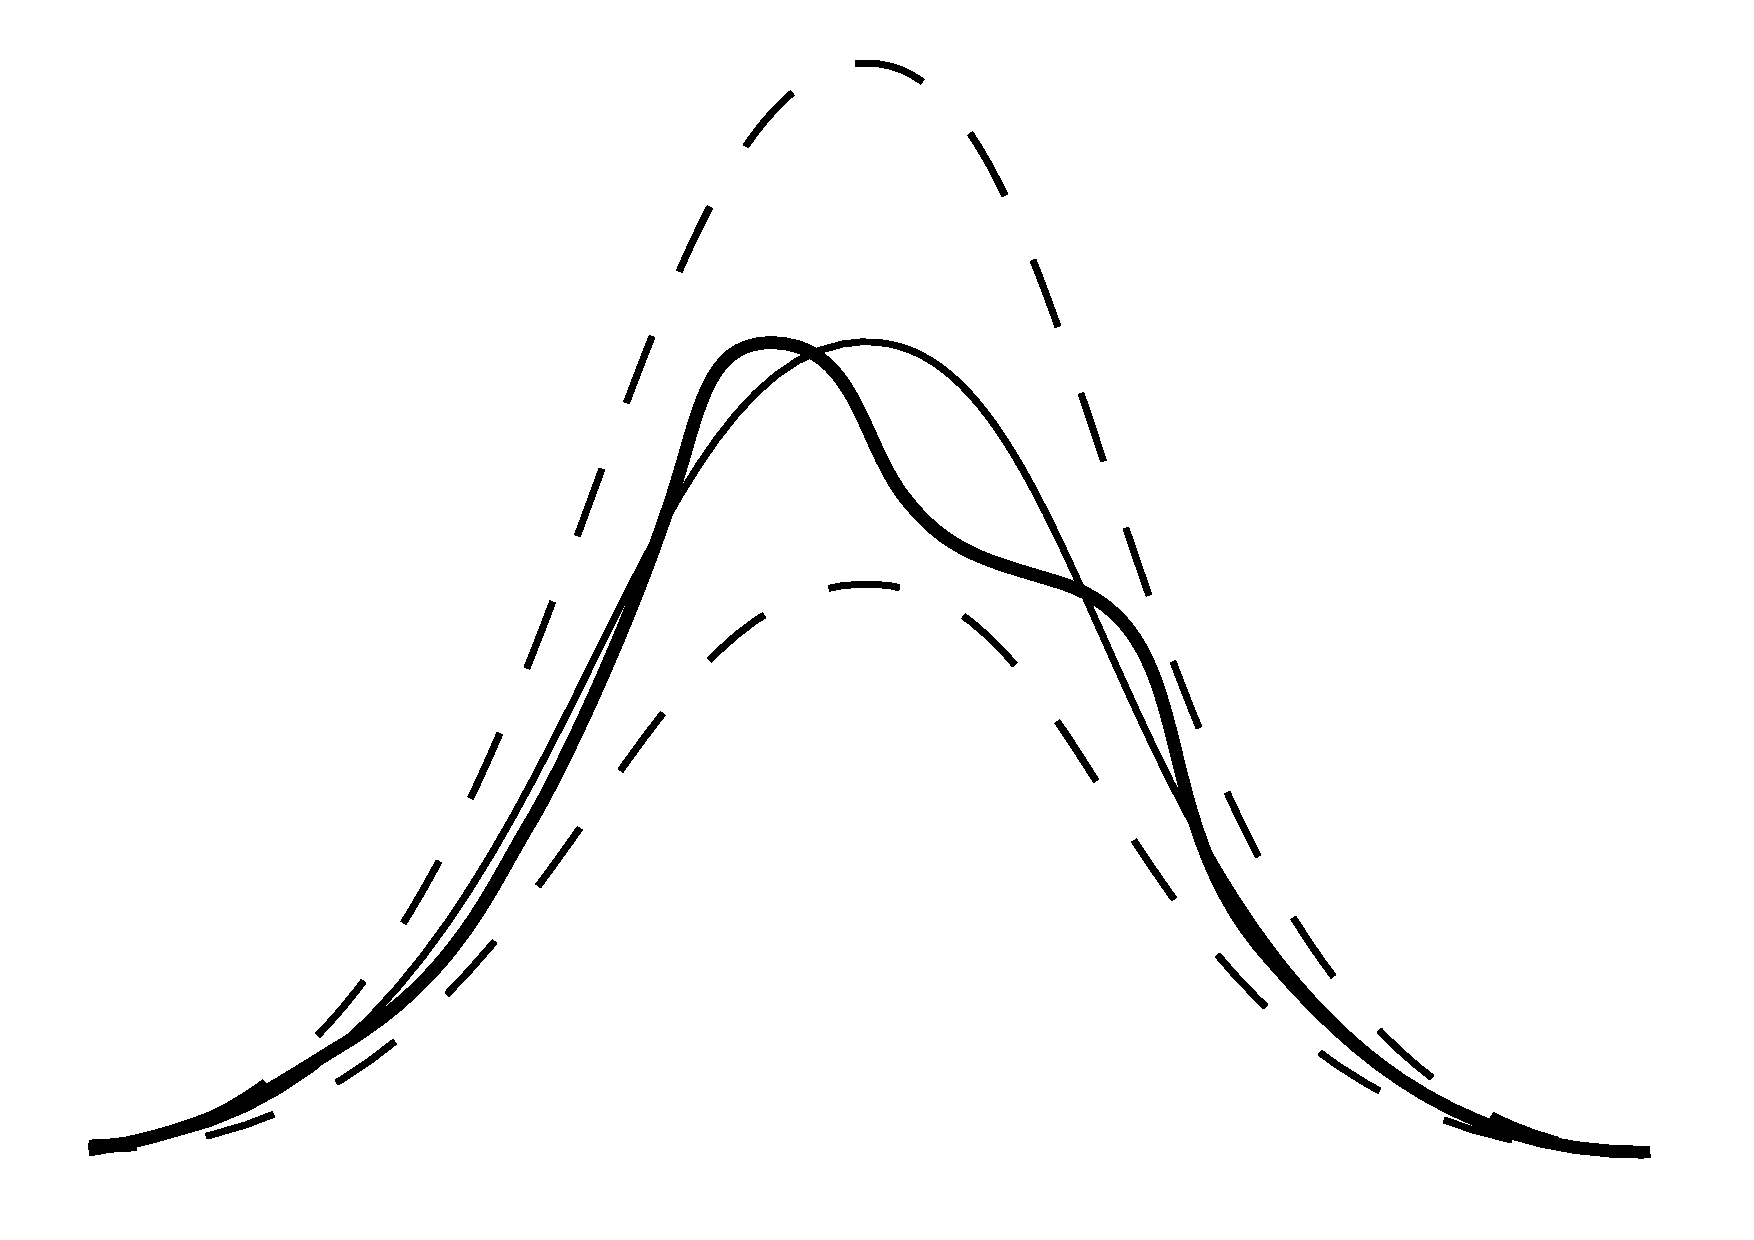
\includegraphics[width=\unitlength,page=1]{./diagrams/py-bounds.pdf}}%
    \put(0.39432495,0.40447998){\Large $\trueProb(\dataVariables)$}%
    \put(0.40333575,0.27675171){\Large $F_C \physicsProb(\dataVariables)$}%
    \put(0.57081228,0.6197671){\Large $\frac{1}{F_G}\physicsProb(\dataVariables)$}%
    \put(0.48646448,0.53538479){\Large $p(\dataVariables)$}%
  \end{picture}%
\endgroup%
    \caption{Visualisation of the lower and upper bound on
      $\trueProb(\dataVariables)$ to highlight how the approximation,
      $\physicsProb(\dataVariables)$, corresponds to the bounds
      combining with the fidelities, $F_C$.}
    \label{fig-py-bounds}
\end{figure}



\begin{figure}
  \centering
  \def\svgwidth{\textwidth}
    %% Creator: Inkscape 1.0.2 (e86c8708, 2021-01-15), www.inkscape.org
%% PDF/EPS/PS + LaTeX output extension by Johan Engelen, 2010
%% Accompanies image file 'log-py-bounds.pdf' (pdf, eps, ps)
%%
%% To include the image in your LaTeX document, write
%%   \input{<filename>.pdf_tex}
%%  instead of
%%   \includegraphics{<filename>.pdf}
%% To scale the image, write
%%   \def\svgwidth{<desired width>}
%%   \input{<filename>.pdf_tex}
%%  instead of
%%   \includegraphics[width=<desired width>]{<filename>.pdf}
%%
%% Images with a different path to the parent latex file can
%% be accessed with the `import' package (which may need to be
%% installed) using
%%   \usepackage{import}
%% in the preamble, and then including the image with
%%   \import{<path to file>}{<filename>.pdf_tex}
%% Alternatively, one can specify
%%   \graphicspath{{<path to file>/}}
%% 
%% For more information, please see info/svg-inkscape on CTAN:
%%   http://tug.ctan.org/tex-archive/info/svg-inkscape
%%
\begingroup%
  \makeatletter%
  \providecommand\color[2][]{%
    \errmessage{(Inkscape) Color is used for the text in Inkscape, but the package 'color.sty' is not loaded}%
    \renewcommand\color[2][]{}%
  }%
  \providecommand\transparent[1]{%
    \errmessage{(Inkscape) Transparency is used (non-zero) for the text in Inkscape, but the package 'transparent.sty' is not loaded}%
    \renewcommand\transparent[1]{}%
  }%
  \providecommand\rotatebox[2]{#2}%
  \newcommand*\fsize{\dimexpr\f@size pt\relax}%
  \newcommand*\lineheight[1]{\fontsize{\fsize}{#1\fsize}\selectfont}%
  \ifx\svgwidth\undefined%
    \setlength{\unitlength}{841.88976378bp}%
    \ifx\svgscale\undefined%
      \relax%
    \else%
      \setlength{\unitlength}{\unitlength * \real{\svgscale}}%
    \fi%
  \else%
    \setlength{\unitlength}{\svgwidth}%
  \fi%
  \global\let\svgwidth\undefined%
  \global\let\svgscale\undefined%
  \makeatother%
  \begin{picture}(1,0.70707071)%
    \lineheight{1}%
    \setlength\tabcolsep{0pt}%
    \put(0,0){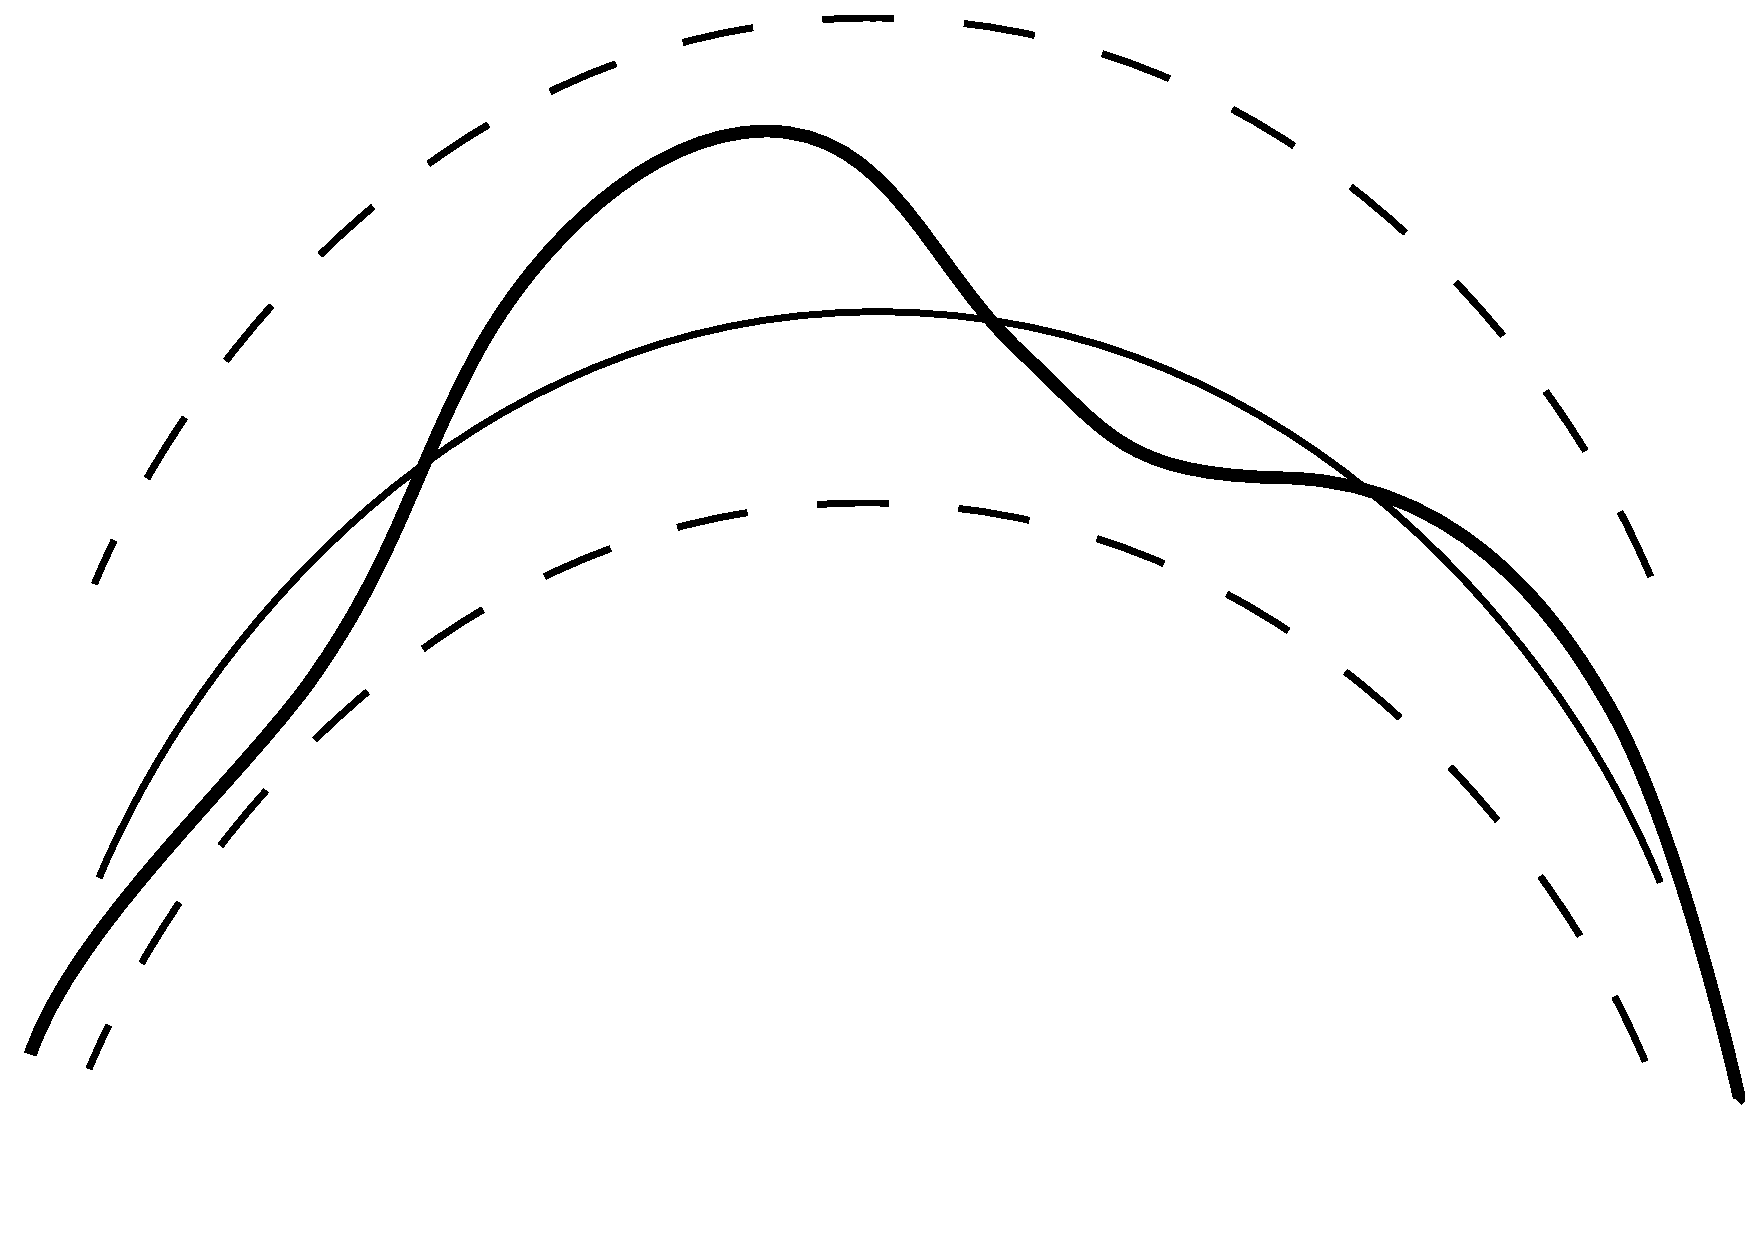
\includegraphics[width=\unitlength,page=1]{./diagrams/log-py-bounds.pdf}}%
    \put(0.55054713,0.58056959){$\log \trueProb(\dataVariables)$}%
    \put(0.31892536,0.34449357){$\log \physicsProb(\dataVariables) + \log F_C$}%
    \put(0.67081228,0.66609147){$\log \physcisProb(\dataVariables) - \log F_G$}%
    \put(0.39197527,0.46832211){$\log \physicsProb(\dataVariables)$}%
  \end{picture}%
\endgroup%

    \caption{Visualisation of the lower and upper bound on $\log
      \trueProb(\dataVariables)$ to highlight how the approximation,
      $\log \physicsProb(\dataVariables)$, corresponds to the bounds
      combining with the fidelities, $\log F_C$ and $\log F_G$.}
    \label{fig-log-py-bounds}
\end{figure}
\subsection{Null Space and Domain Space}

In the scenario as we've laid it out so far is dealing with the number of variables and/or microstates in the universe. But when considering an individual simulation, we don't incorporate all the variables in the universe. There are particular variables we include in our model, and other variables that we choose to ignore. 

We'll introduce this idea into our simulation, $r(\stateVariables)$. We'll introduce two different spaces for our variables. We call the space of variables we'd like to ignore the \emph{null space} and we denote them by $\nullVariables$. The variables of interest we call the \emph{domain space} and we denote by $\domainVariables$.

To build a simulation in practice, we must make some assumptions about the relationship between the null space and the domain space. To see this, let's first of all think of thermodynamic systems. In those systems two different assumptions are common. One approach is to consider an 
\href{https://en.wikipedia.org/wiki/Isolated_system}{\emph{isolated
system}} where no exchange of energy or matter occurs between the null
space and the domain space. In this circumstance, we can ignore the null space and focus only on the domain space. 

\begin{figure}
\missingfigure{Diagram depicting the null space and the domain space.}
\caption{The space of all variables is partitioned into a \emph{null space}, containing $\nullVariables$, and a \emph{domain space}, containing $\domainVariables$.}
\end{figure}

An alternative assumption is to assume that the null
space is a \href{https://en.wikipedia.org/wiki/Thermal_reservoir}{\emph{thermal
resevoir}}.  The idea is that the thermal reservoir is many times larger than the system of interest. So much greater that heat energy may flow from the null space to the domain
space \emph{without} a change in the temperature of the null space.

We represent the microstates of the \emph{null space} as
\(\nullVariables\) and those of the domain space \(\domainVariables\),
\(\stateVariables = \{\nullVariables, \domainVariables\}\). The domain
space contains microstates of interest to our problem, and the null
space contains microstates that are not directly of interest. In
particular the null space contains variables that we believe are only
weakly influenced by our measurements.

We wish to make more general statements about modelling, and so we will take a mathematical approach to separating null and domain spaces. Our approach will be to make a mean field assumption, or \emph{independence} assumption, on the posterior distribution of the null space and the domain space given our observation of $\dataVariables$.

This assumption leads to an approximation for the available energy, allowing us to calculate the apparent available energy without recourse to modelling the entire null space. The approximation mathematically captures both the thermodynamic approaches outlined above, the isolated system and the thermal bath. But it also allows us to examine what happens in our estimates when our independence assumption is violated. In practice, we argue that real-world modelling implicitly makes the same factorisation assumption, but often does it unknowingly. Our more formal approach allows us to capture how a real world model breaks down when the assumptions behind the approximation are violated.

We assume that the distribution of microstates across the two spaces
\emph{factorises}. The factorisation will allow us to explicitly
characterise how our assumption relates to the true system. 

We impose the following constraint on our approximation of the underlying physics, 
\[
\r(\nullVariables, \domainVariables) = r(\nullVariables) r(\domainVariables).
\]

Within the family of physical simulations that are consistent with our constraint, we find the simulation distribution  that minimizes the simulation divergence of the system, \(D_{\stateVariables|\dataVariables}\). To do this we perform a freeform mazimization of the fidelity (see Appendix \ref{sec-free-form-optimization-of-the-domain-space-simulation-distribution}). This gives us the optimal form of the factor representing the domain variables as
\[
r(\domainVariables) = \frac{\exp\left(-\beta E^\prime(\domainVariables)\right)}{Z^\prime_{\domainVariables | \dataVariables}}, 
\] 
where we've introduced a modified Hamiltonian, $E^\prime (\cdot)$ that averages aver the effects of the null space as follows,
\begin{align*}
E^\prime(\domainVariables) = & \expDist{E(\dataVariables |\stateVariables)}{\trueProb(\dataVariables)r(\nullVariables)}+\expDist{E(\stateVariables)}{r(\nullVariables)} \\
Z^\prime_{\domainVariables | \dataVariables} = & \int \exp\left( - \beta E^\prime(\domainVariables)\right) \text{d}\domainVariables. 
\end{align*}

The factor representing the null variables can be found and has a symmetric form (see Appendix \ref{sec-symmetric-form-of-the-null-space-simulation-distribution}).

Note that these two distributions are interdependent. The optimal
form of \(r(\domainVariables)\) is dependent on
the form of \(r(\nullVariables)\) through the modified Hamiltonian. Similarly, the null variable's factor depends on the domain variables through an alternative modified Hamiltonian (see Appendix).

At this point we can see the motivation for the two different modelling assumptions used in thermodynamics. In the isolated system, the posterior over the null space and the domain space genuinely is independent. This independence means that the modified Hamiltonian is equivalent to the original Hamiltonian,
%
\begin{align*}
E^\prime(\domainVariables) \equiv & \expDist{E(\dataVariables |\domainVariables)}{\trueProb(\dataVariables)} +  E(\domainVariables),
\end{align*}
%
and the approximation becomes exact.

The thermal reservoir is somewhat different. The definition of the thermal reservoir is such that it does not change its macroscopic properties in response to changes in the domain variables. This assumption arises from the assumed much larger size of the null space to the domain space. Further, it is only through these macroscopic properties that the reservoir influences the domain space, e.g. in thermodynamics it would be temperature and pressure. So, in the thermal reservoir case, we no longer have $E^\prime(\dataVariables |\domainVariables) = E(\dataVariables |\domainVariables)$, because the null space (i.e. the reservoir) \emph{does} influence the domain space. But the size of this reservoir means that the influence of the null space does \emph{not} change over time as the domain space is updated. So the influence of $r(\nullVariables)$ can be seen as static  and $E^\prime(\dataVariables |\domainVariables)$ can be genuinely seen as a proxy for the true Hamiltonian (even if it is not directly equal to it).  

Our approximation goes beyond the two different cases considered in thermodynamics and also allows us to make more general statements about validity. The isolated system and the thermodynamic bath are two cases where the simulation divergence can be minimized to zero, but in general modelling scenarios we are unlikely to be in either of these two situations. So we may have to interact between updates to the domain space factor and the null space factor to minimize simulation divergence and improve our estimate of the apparent available energy and the intelligence quotient. In this case we can drive the simulation divergence to zero as long as we choose our null space, domain space and observed variables such that the factorise in one of the manners shown in Figure \ref{fig-null-space-factorisation}.

\begin{figure}
    \centering
    \missingfigure{Graphical model showing valid factorizations of the null space and domain space.}
    \caption{Different factorizations of the null space and domain space that allow us to drive the simulation discrimination to zero. In practice definition of the null space and the domain space is a component of our model choice, e.g. we need to decide which features we might include in a neural network classifier. Different choices affect our ability to estimate the intelligence quotient in different ways.}
    \label{fig-null-space-factorisation}
\end{figure}

\todo{Relate to Kullback minimum discriminaton and Jaynes maximum entropy}
The approach of minimising discrimination was proposed by \cite{Kullback-} as minimum discrimination information and by Jaynes as maximum entropy \cite{} \todo{citations to kullback and Jaynes}.

\section{The Data Model}

The factorisation of our simulation distribution allows us to return our attention to the \emph{data model}, $\physicsProb(\dataVariables)$. Recalling the apparent available energy gain, 
\[
\expDist{\Delta A^\prime_{\stateVariables|\dataVariables}}{\trueProb(\dataVariables)} = -\expDist{E(\dataVariables)}{\trueProb(\dataVariables)} + TS^\prime_\dataVariables.
\] 
and re-expanding $E(\dataVariables)$ as 
\[
\expDist{\Delta A^\prime_{\stateVariables|\dataVariables}}{\trueProb(\dataVariables)} = \expDist{E^\prime(\dataVariables|\stateVariables_1)}{\trueProb(\dataVariables)} + -\expDist{E^\prime(\dataVariables|\stateVariables_1)}{\physicsProb(\dataVariables)}+ TS^\prime_\dataVariables.
\] 
an interesting way forward emerges. 

In practice, we do not have access to the true probability distributions, we can only sample from the world, with a corresponding energy cost, $E(\measuredVariables_\dataVariables=\textbf{1})$. This sample of variables is associated with the following apparent change in energy, 
\[
\expDist{\Delta A^\prime_{\stateVariables|\dataVariables}}{\trueProb(\dataVariables)} = \expDist{E^\prime(\dataVariables|\stateVariables_1)}{\physicsProb(\stateVariables_1|\dataVariables)}  -\expDist{E^\prime(\dataVariables|\stateVariables_1)}{\physicsProb(\stateVariables_1|\dataVariables)\physicsProb(\dataVariables)}+ TS^\prime_\dataVariables.
\] 
for simplicity we denote,
\[
f(\dataVariables) = \expDist{E^\prime(\dataVariables|\stateVariables_1)}{\physicsProb(\stateVariables_1|\dataVariables)}.
\]
and now we write
\[
A_{\stateVariables|\dataVariables} = \sum f(\dataVariables) -
\]
The form of our apparent AEG  then we can choose a form for $\physicsProb(\dataVariables)$ that minimizes 
we can look at an empirical estimate by taking 

Recalling that the apparent available energies are written in terms of the partition functions of our simulation,
\begin{align*}
A^\prime_{\stateVariables|\dataVariables_1} & = - \frac{1}{\beta} \log Z_{\stateVariables|\dataVariables_1}^\prime \\
A^\prime_{\stateVariables,\dataVariables_1} & = - \frac{1}{\beta} \log Z_{\stateVariables,\dataVariables_1}^\prime
\end{align*}
we can write down the apparent available energy gain as,
\begin{align*}
\Delta A^\prime_{\stateVariables|\dataVariables_1} & = - \frac{1}{\beta} \log \frac{Z_{\stateVariables|\dataVariables_1}^\prime}{Z_{\stateVariables,\dataVariables_1}^\prime}\\
& = -\frac{1}{\beta} \log \physicsProb(\dataVariables)
\end{align*}
and the apparent intelligence quotient is given by
\[
I^\prime =\frac{\exp\left(-\beta E(\measuredVariables_\dataVariables=\textbf{1})\right)}{\physicsProb(\dataVariables)}
\]
And we note, 
\[
\expDist{\log I}{\trueProb(\dataVariables)} = \expDist{\log I^\prime}{\trueProb(\dataVariables)} - \text{KL}(\trueProb(\dataVariables)||\physicsProb(\dataVariables))
\]
giving 
\[
\expDist{\log I}{\trueProb(\dataVariables)} \leq \expDist{\log I^\prime}{\trueProb(\dataVariables)}
\] 
implying that we can get an upper bound estimate on the expected logarithm of intelligence quotient. The upper bound is tightened by minimising $\text{KL}(\trueProb(\dataVariables)||\physicsProb(\dataVariables))$, or the inclusive KL divergence. 

Conversely, we can lower bound the expected logarithm of the intelligence quotient where the expectation is under $\physicsProb(\dataVariables)$. 
\[
\expDist{\log I}{\physicsProb(\dataVariables)} = \expDist{\log I^\prime}{\physicsProb(\dataVariables)} + \text{KL}(\physicsProb(\dataVariables)||\trueProb(\dataVariables))
\]
implying
\[
\expDist{\log I}{\physicsProb(\dataVariables)} \geq \expDist{\log I^\prime}{\physicsProb(\dataVariables)}
\]

\section{Parameterised Model}

The next step is to include \emph{parameters} with the model. To do this
we first separate a new set of auxiliary variables from the domain
variables,
\(\domainVariables \rightarrow \{\domainVariables, \parameterVector\}\)introduce
a new distribution, \[
\approxProb(\domainVariables, \parameterVector) = \physicsProb(\domainVariables | \parameterVector)\approxProb(\parameterVector)
\] 
\begin{align*}
A^\prime_{\domainVariables|\parameterVector} = & -\frac{1}{\beta} \log \int \exp\left(-\beta E^\prime(\dataVariables |\domainVariables, \parameterVector) - \beta E^\prime(\domainVariables, \parameterVector)\right) \text{d}\domainVariables \text{d}\parameterVector\\
= & -\frac{1}{\beta} \expDist{\log\frac{\exp\left(-\beta E^\prime(\dataVariables |\domainVariables, \parameterVector) - \beta E^\prime(\domainVariables, \parameterVector)\right)}{\approxProb(\domainVariables, \parameterVector)}}{\approxProb(\domainVariables, \parameterVector)} - \frac{1}{\beta} \expDist{\log\frac{\approxProb(\domainVariables , \parameterVector)}{\physicsProb(\domainVariables, \parameterVector | \dataVariables)}}{\approxProb(\domainVariables, \parameterVector)} \\
= & -\frac{1}{\beta} \expDist{\log\frac{\exp\left(-\beta \expDist{E^\prime(\dataVariables |\domainVariables, \parameterVector) - \beta E^\prime(\domainVariables, \parameterVector)\right)}{\physicsProb(\domainVariables | \parameterVector)}}{\approxProb(\parameterVector)}}{\approxProb(\parameterVector)} + \frac{1}{\beta} \expDist{\log \physicsProb(\domainVariables | \parameterVector)}{\approxProb(\domainVariables, \parameterVector)} - \frac{1}{\beta} \expDist{\log\frac{\approxProb(\domainVariables , \parameterVector)}{\physicsProb(\domainVariables, \parameterVector | \dataVariables)}}{\approxProb(\domainVariables, \parameterVector)} \\
= & -\frac{1}{\beta} \expDist{\log\frac{\exp\left(-\beta E^{\prime\prime}(\dataVariables |\parameterVector) - \beta E^{\prime\prime}(\parameterVector)\right)}{\approxProb(\parameterVector)}}{\approxProb(\parameterVector)} + \frac{1}{\beta} \expDist{\expDist{\log \physicsProb(\domainVariables | \parameterVector)}{\physicsProb(\domainVariables | \parameterVector)}}{\approxProb(\parameterVector)} - \frac{1}{\beta} \expDist{\expDist{\log\frac{\physicsProb(\domainVariables | \parameterVector)}{\physicsProb(\domainVariables| \parameterVector , \dataVariables)}}{\physicsProb(\domainVariables | \parameterVector)}}{\approxProb(\parameterVector)} - \frac{1}{\beta}\expDist{\log\frac{\approxProb(\parameterVector)}{\physicsProb(\parameterVector|\dataVariables)}}{\approxProb(\parameterVector)}
\end{align*}

If we define 
\[
\statsProb(\dataVariables | \parameterVector) = \frac{\exp\left(-\beta E^{\prime\prime}(\dataVariables |\parameterVector)\right)}{Z^{\prime\prime}_{\dataVariables | \parameterVector}}
\] 
and 
\[
\statsProb(\parameterVector) = \frac{\exp\left(-\beta E^{\prime\prime}(\parameterVector)\right)}{Z^{\prime\prime}_{\parameterVector}},
\] 
where 
\[
Z^{\prime\prime}_{\dataVariables | \parameterVector} = \int \exp\left(-\beta E^{\prime\prime}(\dataVariables |\parameterVector)\right) \text{d}\dataVariables
\] 
and 
\[
Z^{\prime\prime}_{\parameterVector} = \int \exp\left(-\beta E^{\prime\prime}(\parameterVector)\right) \text{d}\parameterVector
\] 
and 
\[
Z^{\prime\prime}_{\parameterVector|\dataVariables} = \int \exp\left(-\beta E^{\prime\prime}(\dataVariables |\parameterVector)\right)  + \exp\left(-\beta E^{\prime\prime}(\parameterVector)\right) \text{d}\parameterVector
\] 
and we set 
\[
\approxProb(\parameterVector) = \statsProb(\parameterVector |\dataVariables)
\] 
then we have 
\[
A^\prime_{\domainVariables|\parameterVector} = -\frac{1}{\beta} \log  Z^{\prime\prime}_{\parameterVector|\dataVariables} - T\expDist{S^\prime_{\domainVariables | \parameterVector}}{\statsProb(\parameterVector | \dataVariables)} - T\expDist{B_{\domainVariables | \parameterVector}}{\statsProb(\parameterVector | \dataVariables)}  - \frac{1}{\beta}\expDist{\log\frac{\statsProb(\parameterVector|\dataVariables)}{\physicsProb(\parameterVector|\dataVariables)}}{\statsProb(\parameterVector|\dataVariables)},
\] 
where 
\[
B^\prime_{\domainVariables | \parameterVector} = k_B \expDist{\log\frac{\physicsProb(\domainVariables | \parameterVector)}{\physicsProb(\domainVariables| \parameterVector , \dataVariables)}}{\physicsProb(\domainVariables | \parameterVector)}
\] 
so overall we have 
\[
A_{\stateVariables|\dataVariables} = -\frac{1}{\beta} \log  Z^{\prime\prime}_{\parameterVector|\dataVariables} - T\expDist{S^\prime_{\domainVariables | \parameterVector}}{\statsProb(\parameterVector | \dataVariables)} - T\expDist{B^\prime_{\domainVariables | \parameterVector}}{\statsProb(\parameterVector | \dataVariables)}  - TM^\prime_{\parameterVector|\dataVariables} - TS^\prime_{\nullVariables|\dataVariables}- TD_{\stateVariables|\dataVariables},
\] 
where 
\[
M^\prime_{\stateVariables|\dataVariables} =  k_B\expDist{\log\frac{\statsProb(\parameterVector|\dataVariables)}{\physicsProb(\parameterVector|\dataVariables)}}{\statsProb(\parameterVector|\dataVariables)}.
\] 
Collecting terms 
\[
A_{\stateVariables|\dataVariables} = A^{\prime\prime}_{\parameterVector|\dataVariables} - T\left[\expDist{S^\prime_{\domainVariables | \parameterVector}}{\statsProb(\parameterVector | \dataVariables)} + S^\prime_{\nullVariables|\dataVariables}\right]   - T\left[M^\prime_{\parameterVector|\dataVariables} + D_{\stateVariables|\dataVariables} + \expDist{B^\prime_{\domainVariables | \parameterVector}}{\statsProb(\parameterVector | \dataVariables)}\right]
\] 
Or 
\[
A^{\prime\prime}_{\parameterVector|\dataVariables} = A_{\stateVariables|\dataVariables} + T\left[\expDist{S^\prime_{\domainVariables | \parameterVector}}{\statsProb(\parameterVector | \dataVariables)} + S^\prime_{\nullVariables|\dataVariables}\right]  + T\left[M^\prime_{\parameterVector|\dataVariables} + D_{\stateVariables|\dataVariables} + \expDist{B^\prime_{\domainVariables | \parameterVector}}{\statsProb(\parameterVector | \dataVariables)}\right]
\]

\subsection{Speculative on Naming}

Spilt the statistical model mismatch into two terms that represent how
'correct' and how 'consistent' the statistical model is.

Correctness represents the ability of the model to reconstruct the
information about domain variables, \(\domainVariables\), that is
provided by the data, \(\dataVariables\), through the parameters,
\(\parameterVector\), alone. The value of
\(B^\prime_{\domainVariables|\dataVariables}\) increases with
incorrectness.

Consistency reflects how likely different data sets are to give us
different parameters. is the relative entropy (KL divergence) between
the parameters of the statistical model,
\(\statsProb(\parameterVector|\dataVariables)\), and the physical model,
\(\physicsProb(\parameterVector|\dataVariables)\). T

\subsection{Absence of the Bayesian
Controversy}\label{absence-of-the-bayesian-controversy}

While these ideas are normally considered for thermodynamics, they can
also be seen as an attempt to capture the full state of a physical
system through probability. In a classical system, each of these states
is the result of some deterministic (physical) relationship.

The fundamentals of statistical mechanics were derived by physicists and
chemists such as Maxwell, Boltzmann, Gibbs and Helmholtz. In chemistry,
particle theories of matter were uncontroversial, although in physics,
Boltzmann struggled throughout his life to have his fellow physicists
accept these ideas and it wasn't until Einstein formulated Brownian
motion with a particle model\cite{Einstein-brownian05}, introducing
stochasticity to \emph{differential equations} and giving predictions
that were verified by Perrin\cite{Perrin-brownian10}.

\subsection{Thermodynamic Relations}\label{thermodynamic-relations}

The view that Boltzmann was competing with was the positivist view of
physics as a universe of energy, pushed by Mach and others.

The relationship between energy and particles is given through
conservation of energy of the microstates. The total energy of a system
is given by the expected value of those energies under probability
distribution of states. \[
U = \expDist{E(\stateVariables)}{\mathbb{P}(\stateVariables)}
\] Note that this is related to the entropy of
\(\mathbb{P}(\stateVariables)\) 
as follows
\begin{align*} 
U = &
\expDist{E(\stateVariables)}{\mathbb{P}(\stateVariables)}
 = &
-\frac{1}{\beta}\expDist{\log
\mathbb{P}(\stateVariables)}{\mathbb{P}(\stateVariables)}
- \frac{1}{\beta} \log Z
\end{align*} 
where in statistical mechanics we denote \[
TS = -\frac{1}{\beta}\expDist{\log\mathbb{P}(\stateVariables)}{\mathbb{P}(\stateVariables)}
\] 
where \(T\) is the temperature of the system and \(S\) is the
thermodynamic entropy which is given by the probabilistic entropy times
Boltzmann's constant, \(k_B\). For notational convenience the
statistical mechanics temperature is defined as
\(\beta = \frac{1}{T k_B}\), so \(Tk_B = \frac{1}{\beta}\).

So from the probabilistic definition of expected energy, we can see that
the total energy is related to the entropy as follows: 
\[
U = TS + A,
\] 
where 
\[
A = \frac{1}{\beta} \log Z.
\] 
In statistical mechanics this is known as the Helmholtz free energy.
It is the amount of energy available for \textbackslash emph\{work\} or
\textbackslash emph\{Arbeit\} in Helmholtz's original German, thus the
letter \(A\) to denote it.

This decomposition of the joint distribution is a fundamental equation
in statistical mechanics.

In thermodynamics, the state variables, \(\stateVariables\) are often
split into extensive and intensive variables. Extensive variables depend
on the quantity of matter (total mass, volume) and intensive do not
(temperature, density).

\subsection{Machine Learning}\label{machine-learning}

In the world of machine learning, we are more interested in the
separation between states that are observable and states that are
unobservable. The statistical mechanical model we've described doesn't
include measurements. Let's modify the energy function by adding in a
new energy, \(E(\dataVariables | \stateVariables)\), which represents
the interaction between our measurements, \(\dataVariables\), and the
state space \(\stateVariables\).

Now the total energy is given by, 
\[
U_2 = \expDist{E(\dataVariables | \stateVariables)}{\mathbb{P}(\stateVariables| \dataVariables)} + \expDist{E(\stateVariables)}{\mathbb{P}(\stateVariables| \dataVariables)}
\] 
and the Boltzmann distribution for
\(\mathbb{P}(\stateVariables | \dataVariables)\) is given by 
\[
\mathbb{P}(\stateVariables,  \dataVariables) \propto \exp \left(-\beta E(\stateVariables) -\beta E(\dataVariables | \stateVariables)\right),
\] 
where the \(\dataVariables\) are values we observe in the system.

This can be related to the entropy of the system given the measurements
as follows, 
\begin{align*}
U_2 & = \expDist{E(\dataVariables |  \stateVariables)}{\mathbb{P}(\stateVariables |  \dataVariables)} + \expDist{E(\stateVariables)}{\mathbb{P}(\stateVariables | \dataVariables)} \\
& = -\frac{1}{\beta} \expDist{\log \mathbb{P}(\stateVariables | \dataVariables)}{\mathbb{P}(\stateVariables | \dataVariables)} - \frac{1}{\beta}\log Z_2.
\end{align*}
If we define the Helmholtz free energy to be, 
\[
A_2 = -\frac{1}{\beta} \log  Z_2,
\] 
where 
\[
Z_2 = \int \exp \left(-\beta E(\stateVariables) -\beta E(\dataVariables | \stateVariables)\right) \text{d}\stateVariables \text{d}\dataVariables
\] 
then we see that our new entropy term is 
\[
TS_2 = -\frac{1}{\beta} \expDist{\log \mathbb{P}(\stateVariables | \dataVariables)}{\mathbb{P}(\stateVariables | \dataVariables)}.
\]

This can be seen to be related to the original entropy as follows, 
\begin{align*}
TS_1 = & -\frac{1}{\beta} \expDist{\log \mathbb{P}(\stateVariables)}{\mathbb{P}(\stateVariables )} \\
= & -\frac{1}{\beta} \int \mathbb{P}(\dataVariables) \expDist{\log \mathbb{P}(\stateVariables | \dataVariables)}{\mathbb{P}(\stateVariables | \dataVariables)} \text{d}\mathbf{y} - \frac{1}{\beta} \expDist{\log \frac{\mathbb{P}(\stateVariables)}{\mathbb{P}(\stateVariables | \dataVariables)}}{\mathbb{P}(\stateVariables, \dataVariables)}\\
= & -\frac{1}{\beta} \int \mathbb{P}(\dataVariables) \expDist{\log \mathbb{P}(\stateVariables | \dataVariables)}{\mathbb{P}(\stateVariables | \dataVariables)} \text{d}\mathbf{y} + \frac{1}{\beta} \expDist{\log \frac{\mathbb{P}(\stateVariables , \dataVariables)}{\mathbb{P}(\stateVariables)\mathbb{P}(\dataVariables)}}{\mathbb{P}(\stateVariables, \dataVariables)} \\
= & T\expDist{S_2}{\mathbb{P}(\dataVariables)}  + T I,
\end{align*}
where I is the mutual information between \(\dataVariables\) and
\(\stateVariables\), 
\[
I = k_B \expDist{\log \frac{\mathbb{P}(\stateVariables , \dataVariables)}{\mathbb{P}(\stateVariables)\mathbb{P}(\dataVariables)}}{\mathbb{P}(\stateVariables, \dataVariables)}. 
\]

This also allows us to look at 
\begin{align*}
\expDist{U_2}{\mathbb{P}(\dataVariables)} = & \expDist{A_2}{\mathbb{P}(\dataVariables)} +  T\expDist{S_2}{\mathbb{P}(\dataVariables)} \\
= & A_2 + TS_1 - TI.
\end{align*}


So we have \[
\expDist{U_2}{\mathbb{P}(\dataVariables)}- U_1    = \expDist{A_2}{\mathbb{P}(\dataVariables)}  - A_1 - TI
\]

If the measurements in the ML system do not disturb the marginal
distribution, so that
\(\mathbb{P}_2(\stateVariables) = \mathbb{P}_1(\stateVariables)\) then
we have 
\[
\expDist{U_2}{\mathbb{P}(\dataVariables)} = U_1 + \expDist{E(\dataVariables|\stateVariables)}{\mathbb{P}(\dataVariables, \stateVariables)}
\] 
we have 
\[
\expDist{E(\dataVariables|\stateVariables)}{\mathbb{P}(\dataVariables, \stateVariables)}  = \expDist{A_2}{\mathbb{P}(\dataVariables)}  - A_1 - TI
\] 
Which can must be greater or equal to zero so 
\[
\expDist{A_2}{\mathbb{P}(\dataVariables)} \geq A_1 + TI
\] 
so the amount of free energy in the machine learning system is at
least as much as in the original system. The additional available energy
is free energy is now available as 
\[
\]

We also note that 
\[
TS_1  \geq TS_2 + TI
\] 
with equality occurring when the mutual information is zero. So we are
guaranteed to have reduced entropy in the machine learning system as
long as the mutual information between \(\dataVariables\) and
\(\stateVariables\) is greater than zero, in other words,
\(\dataVariables\) and \(\stateVariables\) cannot be \emph{independent}.

Another special case would be when mutual information is maximized,
which would occur if we measure every state variable. In this case we
(check this) \textbf{would expect all entropy to be removed and the
total energy to equal the free energy}.

\subsection{Maximizing the Free Energy}\label{maximizing-the-free-energy}

The sensible strategy for the machine learning scientist is to maximize
the free energy, 
\[
A_2 = -\frac{1}{\beta} \log \int \exp \left(-\beta E(\stateVariables) -\beta E(\dataVariables | \stateVariables)\right) \text{d}\stateVariables \text{d}\dataVariables.
\] 
We can introduce an approximating distribution,
\(p(\dataVariables, \stateVariables)\), that represents our best
understanding of how things interact. This allows us to decompose. 
\begin{align*}
-\frac{1}{\beta} \log \int \exp \left(-\beta E(\stateVariables) -\beta E(\dataVariables | \stateVariables)\right) \text{d}\stateVariables \text{d}\dataVariables = & -\frac{1}{\beta} \int p(\dataVariables, \stateVariables) \log \frac{\exp\left(-\beta E(\stateVariables) -\beta E(\dataVariables | \stateVariables)\right)}{p(\dataVariables, \stateVariables)}\text{d}\stateVariables \text{d}\dataVariables \\
& +\frac{1}{\beta} \int p(\dataVariables, \stateVariables) \log \frac{\mathbb{P}(\dataVariables, \stateVariables)}{p(\dataVariables, \stateVariables)}\text{d}\stateVariables \text{d}\dataVariables. \\
\end{align*}
or for a given observation of \(\dataVariables\) we have, 
\begin{align*}
-\frac{1}{\beta} \log \int \exp \left(-\beta E(\stateVariables) -\beta E(\dataVariables | \stateVariables)\right) \text{d}\stateVariables  = & -\frac{1}{\beta} \int p(\stateVariables| \dataVariables) \log \frac{\exp\left(-\beta E(\stateVariables) -\beta E(\dataVariables | \stateVariables)\right)}{p( \stateVariables| \dataVariables)}\text{d}\stateVariables  \\
& +\frac{1}{\beta} \int p(\stateVariables |\dataVariables) \log \frac{\mathbb{P}(\stateVariables| \dataVariables)}{p(\stateVariables | \dataVariables)}\text{d}\stateVariables. \\
\end{align*}

\begin{align*}
A_2 = & \expDist{E(\stateVariables) +E(\dataVariables | \stateVariables)}{p(\dataVariables, \stateVariables)} \\ 
& - \frac{1}{\beta} \expDist{\log p(\dataVariables, \stateVariables)}{p(\dataVariables, \stateVariables)} \\
& +\frac{1}{\beta} \int p(\dataVariables, \stateVariables) \log \frac{\mathbb{P}(\dataVariables, \stateVariables)}{p(\dataVariables, \stateVariables)}\text{d}\stateVariables \text{d}\dataVariables.
\end{align*}
 reordering as 
\begin{align*}
A_2 + \frac{1}{\beta} \expDist{\log \frac{p(\dataVariables, \stateVariables)}{\mathbb{P}(\dataVariables, \stateVariables)}}{p(\dataVariables, \stateVariables) } = & \expDist{E(\stateVariables) +E(\dataVariables | \stateVariables)}{p(\dataVariables, \stateVariables)} 
+ \frac{1}{\beta} \expDist{\log p(\dataVariables, \stateVariables)}{p(\dataVariables, \stateVariables)}.
\end{align*}
We recognise that the left hand side is the free energy plus a
Kullback-Leibler (KL) divergence between our approximating distribution,
\(p(\dataVariables, \stateVariables)\) and the true distribution
\(\mathbb{P}(\dataVariables, \stateVariables)\). We introduce an
apparent free energy, 
\begin{align*}
\hat{A}_2 = & A_2 + \frac{1}{\beta} \expDist{\log \frac{p(\dataVariables, \stateVariables)}{\mathbb{P}(\dataVariables, \stateVariables)}}{p(\dataVariables, \stateVariables)} \\
= & A_2 + T \text{KL}\left(p(\dataVariables, \stateVariables) || \mathbb{P}(\dataVariables, \stateVariables)\right)
\end{align*}
 which, because the KL divergence is greater than or equal to zero,
shows that the apparent free energy is an \emph{upper bound} on the
actual free energy. The tightness of the bound improves as our
approximation, \(p(\dataVariables, \stateVariables)\) approaches the
truth \(\mathbb{P}(\dataVariables, \stateVariables)\).

The other two terms can be seen to be equivalent to the total energy,
\(U_2\), and the entropy, \(S_2\). But again under the assumed
distribution, \(p(\dataVariables, \stateVariables)\), so we have \[
\hat{U}_2 = \expDist{E(\stateVariables) +E(\dataVariables | \stateVariables)}{p(\dataVariables, \stateVariables)}
\] and \[
T\hat{S}_2 = - \frac{1}{\beta} \expDist{\log p(\dataVariables, \stateVariables)}{p(\dataVariables, \stateVariables)}
\] 
This allows us to write down a new assumed free energy relationship.
\[
\hat{A}_2 = \hat{U}_2 - T\hat{S}_2.
\] 
This is the world that, as modellers, we play with. The total energy
term and the entropy term are now given by our \emph{assumed}
probability distribution for the world,
\(p(\dataVariables, \stateVariables)\). Or in other words by the model
we use. That model is an approximation to the truth,
\(\mathbb{P}(\dataVariables, \stateVariables)\). However, rather
insiduously, the worse our approximation to the truth, the greater the
apparent free energy appears to be. Because the apparent free energy is
an upper bound on the true free energy, we have to be very careful about
model fitting, 
\[
A_2 = \hat{A}_2 - T \text{KL}\left(p(\dataVariables, \stateVariables) || \mathbb{P}(\dataVariables, \stateVariables)\right).
\] 
Normally we would be looking to maximize the free energy, which
minimizes the entropy. But here we have to be careful about direct
maximization, because a high \emph{apparent} free energy can be achieved
with a poor model.

Note also, that traditional approaches to probabilistic model fitting
are often justified by minimization of the KL divergence. But that KL
divergence is the \emph{other way around}. Classical maximum likelihoood
minimizes
\(T \text{KL}\left(\mathbb{P}(\dataVariables, \stateVariables) || p(\dataVariables, \stateVariables)\right)\).
I.e. expectations are taken under the true distribution
\(\mathbb{P}(\dataVariables, \stateVariables)\).

So far, everything we've written about concerns \emph{equilibrium
thermodynamics}. The above laws apply once we have stationary
distributions. In theory, that might take infinite time to occur. If we
only consider equilibrium thermodynamics, we loose the element of time.
Time is just as important as free energy as a resource to preserve. When
building an intelligent system we are very often faced with a time
horizon. Algorithms that require us to compute for many billions of
years to get their answers are not of much use.

\begin{align*}
-\frac{1}{\beta} \log \int \exp \left(-\beta E(\stateVariables) -\beta E(\dataVariables | \stateVariables)\right) \text{d}\stateVariables \text{d}\dataVariables = & -\frac{1}{\beta} \int p(\dataVariables)p(\stateVariables | \dataVariables) \log \frac{\exp\left(-\beta E(\stateVariables) -\beta E(\dataVariables | \stateVariables)\right)}{p(\stateVariables|\dataVariables) }\text{d}\stateVariables \text{d}\dataVariables  \\
& +\frac{1}{\beta} \int p(\dataVariables) p(\stateVariables|\dataVariables) \log \frac{\mathbb{P}( \stateVariables| \dataVariables)}{p( \stateVariables | \dataVariables)}\text{d}\stateVariables \text{d}\dataVariables + \frac{1}{\beta} \int p(\dataVariables)  \log  \mathbb{P}(  \dataVariables) \text{d}\dataVariables.\\
= & -\frac{1}{\beta} \int p(\dataVariables)p(\stateVariables | \dataVariables) \log \frac{\exp\left( -\beta E(\dataVariables | \stateVariables)\right)}{p(\stateVariables|\dataVariables) }\text{d}\stateVariables \text{d}\dataVariables + \int p(\dataVariables) p(\stateVariables|\dataVariables) E(\stateVariables) \text{d}\stateVariables \\
& +\frac{1}{\beta} \int p(\dataVariables) p(\stateVariables|\dataVariables) \log \frac{\mathbb{P}( \stateVariables| \dataVariables)}{p( \stateVariables | \dataVariables)}\text{d}\stateVariables \text{d}\dataVariables + \frac{1}{\beta} \int p(\dataVariables)  \log  \mathbb{P}(  \dataVariables) \text{d}\dataVariables.
\end{align*}


\subsection{Maximizing the Available Energy}\label{maximizing-the-available-energy}

The apparent available energy is given by 
\[
\hat{A}_2 =  \expDist{E(\stateVariables) +E(\dataVariables | \stateVariables)}{p(\dataVariables, \stateVariables)} + \frac{1}{\beta} \expDist{\log p(\dataVariables, \stateVariables)}{p(\dataVariables, \stateVariables)}
\] 
which differs from the true available energy by a KL divergence that
represents the \emph{physical plausibility} of the model,
\(T \text{KL}\left(p(\dataVariables, \stateVariables) || \mathbb{P}(\dataVariables, \stateVariables)\right)\).

\subsubsection{Maximising the Apparent Total Energy}\label{maximising-the-apparent-total-energy}

Our first idea could be to maximise the apparent total energy,
\(\hat{U}_2\). This would require us to have an estimate of what that
total energy is so we would have, 
\[
\hat{E}(\dataVariables, \stateVariables)  \approx E(\stateVariables) + E(\dataVariables | \stateVariables).
\] 
Or more precisely an estimate of the expectations under our joint
distribution. 
\[
\expDist{\hat{E}(\dataVariables, \stateVariables)}{p(\dataVariables, \stateVariables)} \approx \expDist{E(\stateVariables) + E(\dataVariables | \stateVariables)}{p(\dataVariables, \stateVariables)}.
\] 
Maximising the expected total energy could be done through proxies
which relate those energies to actual costs in the real world, so we can
see the approximation
\(\expDist{\hat{E}_2(\dataVariables, \stateVariables)}{p(\dataVariables, \stateVariables)}\)
as an objective to be maximised, or its negative as cost to be
minimized.

Minimizing expected costs is reminiscient of operational research, where
the (often montetary) costs of a process are enumerated, and
optimization algorithms are used to find configurations that minimize
expected cost. Optimizing the total energy in this way is optimal when
there is no uncertainty, i.e. when 
\[
\expDist{\hat{E}(\dataVariables, \stateVariables)}{\mathbb{P}(\dataVariables, \stateVariables)} =  \hat{E}\left(\expDist{\stateVariables}{\mathbb{P}(\dataVariables)}, \expDist{\dataVariables}{\mathbb{P}(\dataVariables)}\right) .
\] 
Because in this case the entropy term can be ignored and the apparent
available energy is equal to the total energy. In this case, our
estimate of the apparent available energy would differ from the true
available energy by the following residual, 
\[
E(\langle\stateVariables\rangle) + E(\langle\dataVariables\rangle | \langle\stateVariables\rangle) - \hat{E}(\langle\dataVariables\rangle | \langle\stateVariables\rangle).
\] But for our focus, when there is uncertainty in the system, we need
to consider the entropy term, \(T\hat{S}_2\).

\subsubsection{Maximum Entropy Distribution}\label{maximum-entropy-distribution}

Maximising the apparent total energy is the most optimistic we can be,
we assume no uncertainty. The most pessimistic we can be would be to
consider the situation where the entropy, \(\hat{S}_2\) is
\emph{maximized}. We can see the maximum apparent total energy as an
optimistic approach, maximising is the other extreme.

The maximum entropy principle \cite{Jaynes-brandeis62} allows us to find a form
for \(p(\dataVariables, \stateVariables)\) that maximises \(T\hat{S}_2\)
while ensuring constraints on the distribution moments match some known
value. Here the idea constraint on moments would be, \[
\expDist{E(\dataVariables | \stateVariables)}{p(\dataVariables, \stateVariables)} = \expDist{E(\dataVariables | \stateVariables)}{\mathbb{P}(\dataVariables, \stateVariables)}.
\] This constraint would recover
\(\mathbb{P}(\dataVariables, \stateVariables)\). This would reflect a
world where we had full knowledge of the physics. In practice, as we
suggested for the maximisation of the apparent total energy, we may 
\[
p(\dataVariables, \stateVariables) \propto \exp(\lambda \hat{E}(\dataVariables, \stateVariables))
\] 
with a partition function of the form 
\[
\hat{Z}_2 = \int \exp(\lambda \hat{E}(\dataVariables , \stateVariables)) \text{d} \dataVariables \text{d} \stateVariables.
\] which implies that, 
\[
\hat{A}_2 = \expDist{E(\stateVariables) +E(\dataVariables | \stateVariables) - \frac{\lambda}{\beta}\hat{E}(\dataVariables, \stateVariables)}{p(\dataVariables, \stateVariables)} - \frac{1}{\beta} \log \hat{Z}_2.
\] 
Which reflects how close our model is to the physical reality. We can
substitute,

\subsection{Recap}\label{recap}

with the different modelling steps we have taken so far, we can relate
the original total energy of the system to our new system as follows, \[
\hat{A}_2 = U_1 + T I(\dataVariables, \stateVariables) + T\text{KL}\left(p(\dataVariables, \stateVariables) || \mathbb{P}(\dataVariables, \stateVariables)\right) - TS_1 - TS_2 - T\hat{S}_2.
\] where we are gaining energy from two sources, firstly through the
information gain from \(\dataVariables\). This is genuine energy gain.
More problematically is the information gain from the KL divergence.
This KL divergence represents the physical plausibility of our model,
\(p(\dataVariables, \stateVariables)\). This is an illusory gain,
because the less physical our model, the more information we seem to
gain. We can immediately see how easy it is to fool ourselves by
building models that don't correspond to the physical reality of our
world.

We are loosing energy due to uncertainty, first of all we loose energy
that corresponds to our ignorance about the phase space,
\(\stateVariables\). Then we loose energy that conforms to our ignorance

We can also see the difference between \(\hat{A}_2\) Laplace's demon can
be seen as relating the total energy to the available enrgy. , these two
terms relate to

\subsection{Computational
Approximations}\label{computational-approximations}

Firstly, let's deal with computational approximations.

Introduce an auxiliary variable to the system, \(\parameterVector\).
Assume we can decompose, 
\[
p(\stateVariables, \dataVariables) = \int p(\dataVariables| p(\stateVariables | \parameterVector) p(\parameterVector) \text{d} \parameterVector
\]

\[
\hat{A}_2 = \expDist{E(\dataVariables , \stateVariables) - \frac{\lambda}{\beta}\hat{E}(\dataVariables, \stateVariables)}{p(\stateVariables | \dataVariables)} - \frac{1}{\beta} \log \hat{Z}_2.
\] 
\begin{align*}
\hat{Z}_2 = & \int \exp\left(\lambda\hat{E}(\dataVariables, \stateVariables)\right) \text{d}\stateVariables\\
= & \int q(\stateVariables, \parameterVector) \log \frac{\exp\left(\lambda\hat{E}(\dataVariables, \stateVariables)\right)p(\stateVariables|\parameterVector) p(\parameterVector)}{q(\stateVariables, \parameterVector)} \text{d}\stateVariables \text{d}\parameterVector+ \int q(\stateVariables, \parameterVector) \log \frac{q(\stateVariables, \parameterVector)p(\dataVariables)}{p(\dataVariables|\stateVariables)p(\stateVariables | \parameterVector)p(\parameterVector)} \text{d}\stateVariables \text{d}\parameterVector
\end{align*}

\begin{align*}
\hat{Z}_2 = & \int \exp\left(\lambda\hat{E}(\dataVariables, \stateVariables)\right) \text{d}\stateVariables\\
= & \int q(\parameterVector) \log \frac{\exp\left(\lambda\hat{E}(\dataVariables, \expDist{\stateVariables}{p(\stateVariables|\parameterVector)})\right)p(\parameterVector)}{q(\parameterVector)} \text{d}\stateVariables \text{d}\parameterVector+ \int q(\stateVariables, \parameterVector) \log \frac{q(\stateVariables, \parameterVector)p(\dataVariables)}{p(\dataVariables|\stateVariables)p(\stateVariables | \parameterVector)p(\parameterVector)} \text{d}\stateVariables \text{d}\parameterVector
\end{align*}

\subsection{Non Equilibrium Thermodynamics}\label{non-equilibrium-thermodynamics}

\subsubsection{Crook's Fluctuation Theorem}\label{crooks-fluctuation-theorem}

Crook's fluctuation theorem \cite{Crooks-fluctuation99} relates the work
done on a system to the free energy difference between the final and
initial state even when the system has not reached equilibrium.

is an equation in statistical mechanics that relates the work done on a
system during a non-equilibrium transformation to the free energy
difference between the final and the initial state of the
transformation. During the non-equilibrium transformation the system is
at constant volume and in contact with a heat reservoir. The CFT is
named after the chemist Gavin E. Crooks (then at University of
California) \cite{Crooks-fluctuation99}.

\bibliography{gibbs-vs-boltzmann}

\appendix

\subsection{Apparent Available Energy Gain}\label{sec-apparent-available-energy-gain}

The apparent available energy gain can be computed as follows:

%
\begin{align*}
A_{\stateVariables|\dataVariables} - A_{\stateVariables,\dataVariables} =  & -\frac{1}{\beta}\expDist{\log \frac{\exp\left(-\beta E(\dataVariables|\stateVariables) -\beta E(\stateVariables)\right)}{\physicsProb(\stateVariables|\dataVariables) }}{\physicsProb(\stateVariables|\dataVariables) } - \frac{1}{\beta}\expDist{\log \frac{\physicsProb(\stateVariables|\dataVariables)}{\trueProb(\stateVariables|\dataVariables) }}{\physicsProb(\stateVariables|\dataVariables) }\\
& +\frac{1}{\beta}\expDist{\log \frac{\exp\left(-\beta E(\dataVariables|\stateVariables) -\beta E(\stateVariables)\right)}{\physicsProb(\stateVariables,\dataVariables) }}{\physicsProb(\stateVariables,\dataVariables) } + \frac{1}{\beta}\expDist{\log \frac{\physicsProb(\stateVariables,\dataVariables)}{\trueProb(\stateVariables,\dataVariables) }}{\physicsProb(\stateVariables,\dataVariables) }
\end{align*} 
Extracting the marginal probabilities of the observations from the final term we can rewrite as 
\begin{align*}
A_{\stateVariables|\dataVariables} - A_{\stateVariables,\dataVariables} =  & -\frac{1}{\beta}\expDist{\log \frac{\exp\left(-\beta \hat{E}(\dataVariables|\stateVariables) -\beta E(\stateVariables)\right)}{\physicsProb(\stateVariables|\dataVariables) }}{\physicsProb(\stateVariables|\dataVariables) } - \frac{1}{\beta}\expDist{\log \frac{\physicsProb(\stateVariables|\dataVariables)}{\trueProb(\stateVariables|\dataVariables) }}{\physicsProb(\stateVariables|\dataVariables) }\\
& +\frac{1}{\beta}\expDist{\log \frac{\exp\left(-\beta E(\dataVariables|\stateVariables) -\beta E(\stateVariables)\right)}{\physicsProb(\stateVariables,\dataVariables) }}{\physicsProb(\stateVariables,\dataVariables) } + \frac{1}{\beta}\expDist{\log \frac{\physicsProb(\stateVariables|\dataVariables)}{\trueProb(\stateVariables|\dataVariables) }}{\physicsProb(\stateVariables,\dataVariables) } + \frac{1}{\beta}\expDist{\log \frac{\physicsProb(\dataVariables)}{\trueProb(\dataVariables) }}{\physicsProb(\dataVariables) }
\end{align*}
We now rewrite in terms of the apparent total energies giving 
\begin{align*}
A_{\stateVariables|\dataVariables} - A_{\stateVariables,\dataVariables} =  & U^\prime_{\stateVariables|\dataVariables} - U^\prime_{\stateVariables,\dataVariables} + TS^\prime_\dataVariables \\
& - \frac{1}{\beta}\expDist{\log\frac{\physicsProb(\stateVariables|\dataVariables)}{\trueProb(\stateVariables|\dataVariables) }}{\physicsProb(\stateVariables|\dataVariables) } \\
 & + \expDist{\frac{1}{\beta}\expDist{\log \frac{\physicsProb(\stateVariables|\dataVariables)}{\trueProb(\stateVariables|\dataVariables) }}{\physicsProb(\stateVariables|\dataVariables) }}{\physicsProb(\dataVariables)}\\
&  + \frac{1}{\beta}\expDist{\log \frac{\physicsProb(\dataVariables)}{\trueProb(\dataVariables) }}{\physicsProb(\dataVariables) }
\end{align*}


\section{Free Form Optimization of the Domain Space Simulation Distribution} \label{sec-free-form-optimization-of-the-domain-space-simulation-distribution}
\todo{Free form optimisation of the domain space distribution description.}

\section{Symmetric form of the Null Space Simulation}\label{sec-symmetric-form-of-the-null-space-simulation}

Similary, 
\[
\physicsProb(\nullVariables|\dataVariables) = \frac{\exp\left(-\beta E^\prime(\dataVariables |\nullVariables) - \beta E^\prime(\nullVariables)\right)}{Z^\prime_{\nullVariables}},
\] 
where 
\begin{align*}
E^\prime(\dataVariables |\nullVariables) = & \expDist{E(\dataVariables |\stateVariables)}{\physicsProb(\domainVariables|\dataVariables)} \\
E^\prime(\nullVariables) = & \expDist{E(\stateVariables)}{\physicsProb(\domainVariables|\dataVariables)} \\
Z^\prime_{\nullVariables | \dataVariables} = & \int \exp\left(-\beta E^\prime(\dataVariables |\nullVariables) - \beta E^\prime(\nullVariables)\right) \text{d}\nullVariables. 
\end{align*}

